\chapter{Methodology}
\chaptermark{Methodology}
\label{ch:Methodology}

A survey of MARL-TSC literature reveals that published methods — IntelliLight \citep{wei2018intellilight}, PressLight \citep{wei2019presslight}, FRAP \citep{zheng2019learning}, CoLight \citep{wei2019colight}, and MPLight \citep{chen2020toward} — all process each agent's local observation through three successive operations, even though individual papers rarely describe their architectures in these unified terms. First, a \emph{local encoder} maps raw traffic measurements to a feature vector capturing demand and phase state at one intersection. Second, an optional \emph{communication layer} aggregates neighbor embeddings over the road graph to introduce spatial context. Third, an \emph{RL optimizer} uses the resulting representation to select a phase and update the policy.

This thesis formalizes that implicit structure as the \textbf{FGS pipeline} (\textbf{F}ramework for \textbf{G}raph-aware \textbf{S}ignal control): a three-module design space in which every MARL-TSC architecture is fully characterized by three independent choices — encoder, communication, and RL algorithm — as illustrated in Figure~\ref{fig:fgs_pipeline}. The FGS pipeline is developed through three generations of iterative diagnosis-and-repair, each addressing a specific module-interface failure identified in evaluation of the preceding design. The final FGS architecture combines FRAP-based action-token encoding, demand-aware GATv2 communication, and a factored neighborhood critic, described in full in Section~\ref{sec:Methodology_FGSArchitecture}.

The remainder of this chapter follows the pipeline structure. Section~\ref{sec:Methodology_ProblemFormulation} states the formal problem. Section~\ref{sec:Methodology_Pipeline} introduces the general framework, its design table, and how prior work maps onto it. Sections~\ref{sec:Methodology_Encoder}--\ref{sec:Methodology_RLModule} describe each module's design choices in depth. Section~\ref{sec:Methodology_FGSArchitecture} describes the FGS pipeline architecture and shared training algorithm. All three variants follow the CTDE paradigm introduced in Section~\ref{sec:TheoreticalBackground_POMDP}: the actor uses only agent $k$'s local observation at execution time, while the centralized critic has access to the joint state during training.

%──────────────────────────────────────────────────────────────────────────────
\section{Problem Formulation}
\label{sec:Methodology_ProblemFormulation}
%──────────────────────────────────────────────────────────────────────────────

A signalized road network with $N$ intersections is modelled as a Decentralized Partially Observable Markov Decision Process (Dec-POMDP) $\langle \mathcal{N}, \mathcal{S}, \{\mathcal{O}_i\}, \{\mathcal{A}_i\}, T, \{r_i\}, \gamma \rangle$, where $\mathcal{N} = \{1, \ldots, N\}$ is the set of agents, $\mathcal{S}$ is the global state of the SUMO environment, $\mathcal{O}_i$ is the local observation space of agent $i$, $\mathcal{A}_i$ is its action space, $T$ is the stochastic transition function determined by the simulator, $r_i$ is the local reward function, and $\gamma \in (0,1)$ is the discount factor. Agents act simultaneously at each decision step; each agent observes only the state of its own intersection and its immediate neighborhood.

%──────────────────────────────────────────────────────────────────────────────
\section{The Three-Module Framework}
\label{sec:Methodology_Pipeline}
%──────────────────────────────────────────────────────────────────────────────
\begin{figure}[t]
\centering
\begin{tikzpicture}[
  envbox/.style={
    rectangle, rounded corners=4pt,
    draw=black!45, fill=gray!8, thick,
    align=center, font=\small\sffamily\bfseries,
    minimum height=1.2cm, minimum width=2.1cm
  },
  modbox/.style={
    rectangle, rounded corners=4pt,
    draw=black!70, fill=white, very thick,
    align=center, font=\small\sffamily\bfseries,
    minimum height=1.2cm, minimum width=2.6cm
  },
  outbox/.style={
    circle,
    draw=black!55, fill=gray!8, thick,
    align=center, font=\normalsize\sffamily\bfseries,
    minimum size=1.0cm
  },
  mainarrow/.style={->, >=Stealth, very thick, black!80, line width=1.4pt},
]

\node[envbox] (env) at (0,   0) {SUMO\\\footnotesize$\mathbf{x}_i \in \mathbb{R}^d$};
\node[modbox] (enc) at (3.0, 0) {Module~I\\\footnotesize Encoder};
\node[modbox] (com) at (6.2, 0) {Module~II\\\footnotesize Communication};
\node[modbox] (rl)  at (9.4, 0) {Module~III\\\footnotesize RL Optimizer};
\node[outbox] (pi)  at (11.6,0) {$\pi_i$};

\draw[mainarrow] (env) -- (enc);
\draw[mainarrow] (enc) -- (com);
\draw[mainarrow] (com) -- (rl);
\draw[mainarrow] (rl)  -- (pi);

\node[font=\scriptsize\itshape, text=gray!65!black] at (3.0, -0.85) {Feature Extraction};
\node[font=\scriptsize\itshape, text=gray!65!black] at (6.2, -0.85) {Feature Sharing};
\node[font=\scriptsize\itshape, text=gray!65!black] at (9.4, -0.85) {Policy Optimization};

\end{tikzpicture}
\caption{The FGS three-module pipeline. Each agent $i$ receives a node feature vector $\mathbf{x}_i \in \mathbb{R}^d$ from the environment. Module~I (Encoder) maps $\mathbf{x}_i$ to a local embedding; Module~II (Communication) propagates embeddings over the road graph; Module~III (RL Optimizer) produces the phase-selection policy $\pi_i$.}
\label{fig:fgs_pipeline}
\end{figure}

\paragraph{Notation.}
Indices $i,j\in\mathcal{N}$ denote intersections; $a,b$ denote phases; $m$ denotes a traffic movement; $k$ identifies the acting agent (the one currently selecting an action). The phase validity flag $m_{i,a}\in\{0,1\}$ equals 1 if phase $a$ is available at intersection $i$ (formally defined in Section~\ref{sec:Methodology_ObservationSpace}). Within the FRAP encoder (Section~\ref{sec:Methodology_FRAP}) the intersection subscript is suppressed. The termination flag in SAC is written $d^{\mathrm{ep}}\in\{0,1\}$ to avoid clash with the observation dimension $d$. Concatenation is $[\,\cdot\;\Vert\;\cdot\,]$. Table~\ref{tab:notation} lists principal intermediate features.

\begin{table}[ht]
  \centering
  \caption{Principal feature symbols used in this chapter. Each symbol is first introduced in the cited equation or section.}
  \label{tab:notation}
  \small
  \setlength{\tabcolsep}{5pt}
  \begin{tabular}{clll}
    \toprule
    \textbf{Symbol}           & \textbf{Shape}     & \textbf{Description}                & \textbf{First defined}                         \\
    \midrule
    $\mathbf{x}_i$            & $\mathbb{R}^d$     & Raw node feature vector             & Eq.~\ref{eq:node_feature}                      \\
    $m_{i,a}$                 & $\{0,1\}$          & Phase validity flag                 & Sec.~\ref{sec:Methodology_ObservationSpace}    \\
    $\mathbf{h}_i$            & $\mathbb{R}^{d_h}$ & Local embedding (FGS Module~I)      & Sec.~\ref{sec:Methodology_MLP}                 \\
    $\boldsymbol{\phi}_{i,a}$ & $\mathbb{R}^C$     & Per-phase demand embedding (FRAP)   & Eq.~\ref{eq:frap_phase_emb}                    \\
    $\mathbf{z}_{i,a}$        & $\mathbb{R}^{d_z}$ & Per-phase action token (FGS Module~I)   & Eq.~\ref{eq:fgsv2_token}    \\
    $\mathbf{d}_i$            & $\mathbb{R}^{d_c}$ & Demand comm.\ embedding (FGS Module~II) & Eq.~\ref{eq:fgsv3_demand}   \\
    $\mathbf{g}_i$            & $\mathbb{R}^{d_c}$ & Gated graph context (Module~II out)     & Eq.~\ref{eq:fgsv3_gate}     \\
    $\alpha_{ij}$             & $\mathbb{R}$       & GATv2 attention weight              & Eq.~\ref{eq:gatv2_attn}                        \\
    $\alpha$                  & $\mathbb{R}_{>0}$  & SAC temperature                     & Eq.~\ref{eq:sac_objective}                     \\
    $d^{\mathrm{ep}}$         & $\{0,1\}$          & Episode-termination flag            & Eq.~\ref{eq:sac_td_target}                     \\
    \bottomrule
  \end{tabular}
\end{table}

Figure~\ref{fig:fgs_pipeline} depicts the general framework. At each decision step, SUMO emits a graph-structured observation $o_i$ for each agent $i$; the node feature vector $\mathbf{x}_i \in \mathbb{R}^d$ is one component of $o_i$ (see Eq.~\ref{eq:node_feature}). The three modules process it sequentially.

Table~\ref{tab:pipeline_design_space} maps representative prior methods and the three FGS instantiations onto this design space. Every prior graph-based method (CoLight) uses GAT with an MLP encoder and DQN; every method using a phase-competition encoder (standalone FRAP) uses no graph communication. No prior work treats all three module choices as variables and ablates their interactions on German RESCO scenarios — that systematic characterization is the primary contribution of this thesis.

\begin{table}[ht]
\centering
\caption{MARL-TSC methods mapped onto the three-module pipeline. Bold rows: proposed methods. ``FRAP-tok.'' = FRAP encoder tapped to produce per-phase action tokens rather than scalar scores. ``GATv2(D)'' = GATv2 operating on demand-derived embeddings (FGS, the final design).}
\label{tab:pipeline_design_space}
\small
\setlength{\tabcolsep}{6pt}
\renewcommand{\arraystretch}{1.15}
\begin{tabular}{lccc}
\toprule
\textbf{Method} & \textbf{Module~I: Encoder} & \textbf{Module~II: Comm.} & \textbf{Module~III: RL} \\
\midrule
IntelliLight \citep{wei2018intellilight}  & MLP         & None  & DQN \\
PressLight \citep{wei2019presslight}      & Pressure    & None  & DQN \\
FRAP \citep{zheng2019learning}            & FRAP        & None  & DQN \\
CoLight \citep{wei2019colight}            & MLP         & GAT   & DQN \\
MPLight \citep{chen2020toward}            & Pressure    & None  & DQN \\
IDQN / IPPO (RESCO baselines)             & MLP         & None  & DQN / PPO \\
\midrule
\textbf{FGS (this thesis)}     & MLP \emph{or} FRAP & GATv2       & SAC \emph{or} PPO \\
\textbf{FGSv2 (this thesis)}   & FRAP-tok.          & GATv2       & SAC \\
\textbf{FGSv3 (this thesis)}   & FRAP-tok.          & GATv2(D)    & SAC \emph{or} PPO \\
\bottomrule
\end{tabular}
\end{table}

%──────────────────────────────────────────────────────────────────────────────
\section{Module~I: Local Encoder}
\label{sec:Methodology_Encoder}
%──────────────────────────────────────────────────────────────────────────────

The encoder converts the raw traffic observation at one intersection into a fixed-length feature vector — the local embedding that will either be passed directly to the RL module (no communication) or sent as a message to neighboring agents. The design choice here is what structural inductive bias to embed in the encoder: an unstructured MLP that learns features from data, or the FRAP competition encoder that makes phase urgency explicit.

\subsection{Observation Space}
\label{sec:Methodology_ObservationSpace}

Each agent receives a dictionary observation at every decision step. The dictionary encodes the agent's local traffic state together with the graph structure of the surrounding network, allowing the model to perform graph message passing during the forward pass.

The node feature matrix $\mathbf{X} \in \mathbb{R}^{N \times d}$ stacks the feature vector of every agent in the network. For agent $i$, the feature vector is
\begin{equation}
  \mathbf{x}_i =
    \bigl[\,\mathbf{e}_{\mathrm{phase}}^{(i)},\;
           t_{\mathrm{green}}^{(i)},\;
           \boldsymbol{\rho}^{(i)},\;
           \mathbf{q}^{(i)}\,\bigr] \in \mathbb{R}^{d},
  \label{eq:node_feature}
\end{equation}
where $\mathbf{e}_{\mathrm{phase}}^{(i)}$ is a one-hot vector encoding the current active phase, $t_{\mathrm{green}}^{(i)}\in\{0,1\}$ indicates whether the minimum green time has been satisfied at intersection $i$ \citep{wei2018intellilight}, and $\boldsymbol{\rho}^{(i)}, \mathbf{q}^{(i)}$ are the lane density and lane queue vectors over all incoming lanes of intersection $i$.

The remaining fields in the observation dictionary are:
\begin{itemize}
  \item \textit{Edge index} $\mathcal{E} \in \mathbb{Z}^{2 \times |\mathcal{E}|}$: source--target integer pairs defining the agent communication graph.
  \item \textit{Edge mask} and \textit{edge weight}: a binary validity flag and a scalar weight $w_{ij}$ for each edge (see Section~\ref{sec:Methodology_DataPreprocessing}).
  \item \textit{Ego index}: the integer identifying which row of $\mathbf{X}$ corresponds to the acting agent.
  \item \textit{Action mask} $\mathbf{m}_i \in \{0,1\}^{A_{\max}}$: component $m_{i,a}=1$ if phase $a$ is valid at intersection $i$, and 0 otherwise. When the intersection subscript is omitted (e.g., in the FRAP and FGS actor derivations) agent $k$ is implied.
  \item \textit{Phase-pair mask} $\mathbf{M}_{\mathrm{pair}} \in \{0,1\}^{N \times A_{\max} \times M}$: for each agent and candidate phase, indicates the subset of traffic movements that phase controls.
  \item \textit{Phase-competition mask} $\mathbf{M}_{\mathrm{comp}} \in \{0,1,2,3\}^{N \times A_{\max} \times (A_{\max}-1)}$: encodes one of four movement-conflict relation types between phase $a$ and each competitor $b$, following the FRAP relation taxonomy \citep{zheng2019learning}: type~0 — no shared movement conflicts (non-competing phases); type~1 — one shared conflicting movement; type~2 — two shared conflicting movements; type~3 — the phases serve directly opposing movements on the same approach. The self-competition entry is absent by construction.
  \item \textit{Previous joint action} $\mathbf{a}_{t-1} \in \{0,1\}^{N \times A_{\max}}$: one-hot encoding of all agents' actions at the preceding step. This field provides each agent with knowledge of the phase active at neighboring intersections at the prior step, supporting the demand-aware coordination in FGS (Section~\ref{sec:Methodology_FGSArchitecture}).
\end{itemize}

\subsection{MLP Encoder}
\label{sec:Methodology_MLP}

The simplest encoder choice is a shared two-layer MLP that maps the raw feature vector $\mathbf{x}_i \in \mathbb{R}^d$ to a local embedding $\mathbf{h}_i \in \mathbb{R}^{d_h}$:
\[
  \mathbf{h}_i = \mathrm{MLP}_\psi(\mathbf{x}_i), \quad i = 1,\ldots,N.
\]
The MLP encoder treats the observation as an unstructured vector with no prior knowledge about which features correspond to which phases or movements. This is the most common encoder choice in MARL-TSC literature — used in IntelliLight \citep{wei2018intellilight}, CoLight \citep{wei2019colight}, and RESCO baselines \citep{ault2021reinforcement} — and it serves as the baseline against which the FRAP encoder is compared in the FGS ablation study.

\subsection{FRAP Encoder}
\label{sec:Methodology_FRAP}

FRAP \citep{zheng2019learning} encodes the competition between candidate signal phases by explicitly comparing each phase against every competitor and pooling the results. It embeds the core domain insight that the controller's decision reduces to a relative question: \emph{which candidate phase has the most urgent demand compared with the movements it preempts?} By making this comparison explicit in the architecture, FRAP acts as a structured inductive bias that reduces the number of samples needed to learn effective phase selection. Throughout this section the intersection subscript $i$ is suppressed for clarity; all tensors and indices belong to a single intersection.

Let the intersection have $M$ incoming traffic movements and $A$ candidate phases. The phase-movement mask $\mathbf{P} \in \{0,1\}^{A \times M}$ sets $P_{am}=1$ if movement $m$ is served by phase $a$. The phase-competition relation $R_{ab} \in \{0,1,2,3\}$ encodes one of four movement-conflict types between each ordered pair $(a, b)$ of distinct phases, as defined in Section~\ref{sec:Methodology_ObservationSpace} (types~0--3 range from no shared conflict to directly opposing movements).

\paragraph{Step 1: Movement embedding.}
For each movement $m$, a phase indicator $p_m\in\{0,1\}$ (whether $m$ is currently green) and a demand scalar $d_m$ (lane queue length or vehicle density) are embedded separately and fused:
\begin{equation}
  \mathbf{e}_m =
    \operatorname{ReLU}\!\Bigl(
      W_{\text{lane}}\bigl[
        \sigma\!\bigl(\operatorname{Emb}_p(p_m)\bigr),\;
        \sigma(W_d\,d_m)
      \bigr]
    \Bigr) \in \mathbb{R}^{C},
  \label{eq:frap_movement_emb}
\end{equation}
where $\operatorname{Emb}_p\in\mathbb{R}^{2\times C}$ is a two-entry learnable lookup table \citep{zheng2019learning}: embedding the binary indicator rather than passing $p_m$ directly as a scalar gives the model an unconstrained $C$-dimensional representation of the serving and non-serving states, instead of forcing them to map to a fixed numeric ratio; $W_d$ is a demand projection; and $\sigma$ is the sigmoid function.

\paragraph{Step 2: Phase embedding.}
For each candidate phase $a$, the movement embeddings of the movements it controls are aggregated via a scaled sum:
\begin{equation}
  \boldsymbol{\phi}_a = \sum_{m=1}^{M} w_{am}\,\mathbf{e}_m \in \mathbb{R}^{C},
  \label{eq:frap_phase_emb}
\end{equation}
where $P_{am}\in\{0,1\}$ is the entry of the phase-movement mask $\mathbf{P}$ indicating whether movement $m$ is served by phase $a$ (defined above). In the original FRAP formulation \citep{zheng2019learning} $w_{am} = P_{am}$, which assumes every phase controls exactly two movements. German RESCO intersections have variable movement counts per phase, so this implementation replaces the plain mask with a scaled weight:
\begin{equation}
  w_{am} = P_{am}\cdot\frac{\min\!\bigl(\textstyle\sum_{m'} P_{am'},\;2\bigr)}{\max\!\bigl(\textstyle\sum_{m'} P_{am'},\;1\bigr)},
  \label{eq:frap_weight}
\end{equation}
which rescales $\boldsymbol{\phi}_a$ to the equivalent of a two-movement sum regardless of how many movements phase $a$ controls, ensuring scale comparability across heterogeneous phases. The vector $\boldsymbol{\phi}_a$ is also used by FGS as the demand communication signal (Section~\ref{sec:Methodology_FGSArchitecture}).

\paragraph{Step 3: Pairwise competition feature.}
For each ordered competitor pair $(a, b)$ with $b \ne a$:
\begin{align}
  \mathbf{h}_{ab} &=
    \operatorname{ReLU}\!\bigl(
      \operatorname{Conv}_{\text{pair}}\bigl([\boldsymbol{\phi}_a \;\Vert\; \boldsymbol{\phi}_b]\bigr)
    \bigr) \in \mathbb{R}^{C}, \label{eq:frap_h} \\
  \mathbf{r}_{ab} &=
    \operatorname{ReLU}\!\bigl(
      \operatorname{Conv}_{\text{rel}}\bigl(\operatorname{Emb}_{\text{rel}}(R_{ab})\bigr)
    \bigr) \in \mathbb{R}^{C}, \label{eq:frap_r} \\
  \mathbf{c}_{ab} &=
    \operatorname{ReLU}\!\bigl(
      \operatorname{Conv}_{\text{hid}}\bigl(\mathbf{h}_{ab} \odot \mathbf{r}_{ab}\bigr)
    \bigr) \in \mathbb{R}^C. \label{eq:frap_c}
\end{align}
The relation embedding $\mathbf{r}_{ab}$ captures the movement-conflict type; the Hadamard product\footnote{The Hadamard product $\odot$ denotes element-wise multiplication: $\begin{pmatrix}a\\b\end{pmatrix}\odot\begin{pmatrix}c\\d\end{pmatrix}=\begin{pmatrix}ac\\bd\end{pmatrix}$, or for $2\times2$ matrices, $\begin{pmatrix}a&b\\c&d\end{pmatrix}\odot\begin{pmatrix}e&f\\g&h\end{pmatrix}=\begin{pmatrix}ae&bf\\cg&dh\end{pmatrix}$.} gates the phase-pair interaction by this structure. The vector $\mathbf{c}_{ab}$ is the \emph{phase-competition representation} — a per-competitor feature encoding both relative demand and structural conflict.

\paragraph{Step 4: Phase score (original FRAP output).}
In the original FRAP, a final $1{\times}1$ convolution projects each competition feature to a scalar:
\begin{equation}
  s_{ab} = \operatorname{Conv}_{1\times1}(\mathbf{c}_{ab}) \in \mathbb{R}.
  \label{eq:frap_scalar}
\end{equation}
The phase score for candidate phase $a$ is obtained by summing over all valid competitors $V_a = \{b \mid b\ne a,\, m_b=1\}$ (suppressing the intersection subscript as above):
\begin{equation}
  s_a = \sum_{b \in V_a} s_{ab},
  \label{eq:frap_score}
\end{equation}
yielding one scalar per candidate phase that directly serves as a Q-value estimate in the original FRAP policy.

FGS \emph{replaces} Step~4 entirely: instead of projecting $\mathbf{c}_{ab}$ to a scalar, it mean-pools $\mathbf{c}_{ab}$ across valid competitors to produce a per-phase action token $\mathbf{z}_{i,a}$ (Eq.~\ref{eq:fgsv2_token}; intersection subscript $i$ restored), which is then consumed directly by the action-conditioned actor (Eq.~\ref{eq:fgsv2_actor}). This retains the full $C$-dimensional feature vector through Module~II and Module~III without discarding per-phase competition information.

The overall design is permutation-equivariant with respect to phase ordering: reordering the candidate phases produces a correspondingly reordered output vector, which supports generalization across intersections with heterogeneous phase counts and movement configurations.

%──────────────────────────────────────────────────────────────────────────────
\section{Module~II: Graph Communication}
\label{sec:Methodology_Communication}
%──────────────────────────────────────────────────────────────────────────────

The communication module aggregates neighbor embeddings over the road graph, giving each agent access to spatially correlated demand signals from nearby intersections. Without this module, agents act independently with no knowledge of upstream or downstream conditions — the baseline used by IDQN and IPPO. The design choice is the attention mechanism: fixed-weight aggregation, static GAT (CoLight), or dynamic GATv2 (this work).

\subsection{Agent Communication Graph}
\label{sec:Methodology_DataPreprocessing}

The agent communication graph $\mathcal{G} = (\mathcal{V}, \mathcal{E}, \mathbf{W})$ is derived from the SUMO road network file (\texttt{.net.xml}) before training begins and is fixed throughout.

\paragraph{Node extraction.}
Every junction that carries a traffic light logic (\texttt{tlLogic}) in the network XML is added to $\mathcal{V}$ as a graph node. Its geographic coordinates are recorded for visualization but are not used as model inputs.

\paragraph{Super-edge construction.}
For each outgoing road segment from a traffic light node, a Dijkstra traversal follows legal road transitions until it reaches the nearest downstream traffic light node, accumulating the intermediate edges along the path. This yields a set of \emph{super-edges} that connect pairs of signalized intersections directly, abstracting away unsignalized junctions in between.

\paragraph{Edge weight assignment.}
The weight of super-edge $(i, j)$ is
\begin{equation}
  w_{ij} = \frac{1}{\tau_{ij}},
  \label{eq:edge_weight}
\end{equation}
where $\tau_{ij}$ is the estimated travel time along the path. When multiple parallel routes connect the same signal pair, their weights accumulate additively. All edges are inserted bidirectionally to enable symmetric message passing. The resulting graph is serialized to disk as a pre-processing artefact and loaded once per training run, adding no per-step overhead. The full extraction procedure is given in Algorithm~\ref{alg:tls_graph} (Appendix~\ref{sec:Appendix_TLSGraphExtraction}).

Figure~\ref{fig:scenario_topologies} shows the extracted agent communication graphs for all six German RESCO scenarios, grouped by tier. Edge width is proportional to the weight $w_{ij} = 1/\tau_{ij}$: thicker edges indicate shorter inter-signal travel times and thus stronger potential influence.

\begin{figure}[ht]
  \centering
  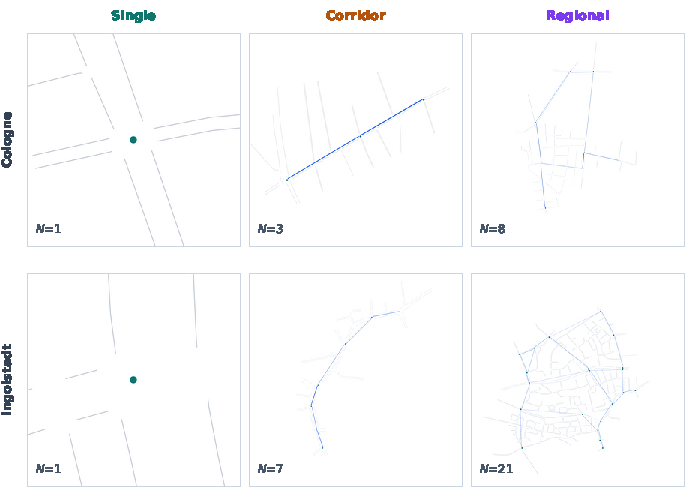
\includegraphics[width=\textwidth]{Figures/scenario_topologies}
  \caption{Agent communication graphs $\mathcal{G}$ for all six German RESCO scenarios. Rows correspond to cities (Cologne, Ingolstadt); columns to scale tiers (Single, Corridor, Regional). Gray polylines show the underlying SUMO road network; blue edges are super-edges between the nearest downstream signalized intersections; green nodes are TLS agents. $N$ denotes the agent count.}
  \label{fig:scenario_topologies}
\end{figure}

\subsection{GATv2 Attention}
\label{sec:Methodology_GAT}

Both FGS and FGSv2 use GATv2 \citep{brody2022how} as the graph communication operator. As discussed in Sections~\ref{sec:TheoreticalBackground_GATv2} and~\ref{sec:LiteratureReview_GraphMLVariants}, GATv2 addresses the static-attention limitation of the original GAT by inserting a non-linearity before the attention scoring, enabling attention coefficients to depend jointly on both the source and the target node's features. The normalized attention coefficient for edge $(i,j)$ is
\begin{equation}
  \alpha_{ij} =
    \frac{
      \exp\!\left(\mathbf{a}^\top \mathrm{LeakyReLU}\!\left(\mathbf{W}\,[\mathbf{h}_i \,\Vert\, \mathbf{h}_j]\right)\right)
    }{
      \sum_{k \in \mathcal{N}(i)}
      \exp\!\left(\mathbf{a}^\top \mathrm{LeakyReLU}\!\left(\mathbf{W}\,[\mathbf{h}_i \,\Vert\, \mathbf{h}_k]\right)\right)
    },
  \label{eq:gatv2_attn}
\end{equation}
where $\mathbf{W}$ and $\mathbf{a}$ are learnable parameters, $\Vert$ denotes concatenation, and $\alpha_{ij}$ is the normalized attention coefficient for edge $(i,j)$ — note that $\alpha_{ij}$ here is a graph-attention weight, distinct from the SAC temperature scalar $\alpha$ used in Section~\ref{sec:Methodology_SAC}. Multi-head attention is applied with $H$ heads; outputs are concatenated and projected to the output dimension. All FGS and FGSv2 variants with graph communication use GATv2 as specified above. A proof of node-permutation equivariance and a discussion of edge-weight integration are in Appendix~\ref{sec:Appendix_GATv2_properties}.

%──────────────────────────────────────────────────────────────────────────────
\section{Module~III: RL Optimizer}
\label{sec:Methodology_RLModule}
%──────────────────────────────────────────────────────────────────────────────

The RL module receives the encoder embedding (optionally enriched by graph communication) and learns a phase-selection policy by optimizing a scalar reward signal. The design choice here spans both the action formulation and the RL algorithm. FGS uses discrete phase selection and evaluates three RL algorithms: DQN, PPO, and SAC. The reward signal is fixed across all methods to isolate algorithmic differences.

\subsection{Action Space}
\label{sec:Methodology_ActionSpace}

The action space of each agent is discrete: at each step the agent selects a phase index from the set of phases its intersection supports. Because intersections in the German RESCO scenarios have different numbers of phases, the action space is padded to a uniform width $A_{\max} = \max_{i \in \mathcal{N}} |\mathcal{A}_i|$. During the forward pass, the logits of all invalid phases are masked to $-\infty$ before the softmax, ensuring that the sampled action always lies within the agent's valid phase set.

Phase transition constraints (minimum green time, yellow interval) are enforced at the SUMO environment level and are not modelled as RL constraints.

\subsection{Reward Function}
\label{sec:Methodology_Rewards}

\subsubsection{Differential Waiting Time}
\label{sec:Methodology_DiffWaitingTime}

All experiments use the differential waiting time reward introduced by the RESCO benchmark \citep{ault2021reinforcement}, defined as the signed change in accumulated waiting time between consecutive decision steps. Cabrejas-Egea et al.\ \citep{cabrejas2020assessment} compare several RL-TSC reward formulations under real-world limitations and find that difference-based waiting-time signals provide stable gradients across varied demand conditions, supporting its adoption here.
\begin{equation}
  r_t = W_{t-1} - W_t,
  \qquad
  W_t = \frac{1}{100}\sum_{l \in \mathcal{L}}\sum_{v \in l} w_v(t),
  \label{eq:reward}
\end{equation}
where $\mathcal{L}$ is the set of incoming lanes controlled by the traffic signal, $v$ indexes vehicles, and $w_v(t)$ is the accumulated waiting time of vehicle $v$ at step $t$ as reported by SUMO via the TraCI interface. The term \emph{differential} follows RESCO's \texttt{diff-waiting-time} naming convention and refers to the finite difference $W_{t-1} - W_t$, not a calculus derivative. A positive value of $r_t$ indicates that total waiting time at the intersection decreased relative to the previous step. Dividing by 100 normalizes the scale across scenarios that differ in traffic volume. Appendix~\ref{sec:Appendix_reward_telescope} proves that maximizing the discounted sum of this reward is equivalent to minimizing a discounted sum of waiting times.

This reward is local to each agent, which aligns with the CTDE assumption: the reward does not require knowledge of the global joint state at execution time, so decentralized policies remain valid after training.

\subsubsection{Alternative Reward Signals}
\label{sec:Methodology_AltRewards}

\paragraph{Delay.}
Delay quantifies the additional travel time incurred by vehicles relative to their free-flow speed. It captures network-level throughput effects directly but requires per-vehicle free-flow speed estimates from SUMO, increasing per-step computational cost. Delay is used as an \emph{evaluation metric} (Section~\ref{sec:ExperimentalDesign_MetricsProcedure}) rather than a training signal.

\paragraph{Pressure.}
Pressure \citep{wei2019presslight} measures the lane imbalance at an intersection:
\begin{equation}
  p_i = \left|\,\sum_{l \in \mathcal{L}_{\mathrm{in}}^{i}} \rho_l
              - \sum_{l \in \mathcal{L}_{\mathrm{out}}^{i}} \rho_l\,\right|,
\end{equation}
where $\rho_l$ is vehicle density on lane $l$. The pressure reward $r_t = -p_i(t)$ penalizes queue accumulation and has been shown to stabilize single-agent training \citep{wei2019presslight}. It was evaluated as an alternative signal but not adopted as the primary reward in this work.

\subsection{DQN and PPO Baselines}
\label{sec:Methodology_ModelsAlgorithmsFrameworks}

The following algorithms serve as baselines or as the algorithmic foundation of the proposed framework. In the multi-intersection setting, each intersection runs an independent copy of the single-agent algorithm with no inter-agent communication. Following the RESCO benchmark terminology \citep{ault2021reinforcement}, the independent-agent variant of DQN is referred to as \textbf{IDQN} (Independent DQN) and the independent-agent variant of PPO is referred to as \textbf{IPPO} (Independent PPO).

\subsubsection{Deep Q-Network}
\label{sec:Methodology_DQN}

Deep Q-Network (DQN) \citep{mnih2015humanlevel} approximates the action-value function with a neural network $Q_\theta(s, a)$ trained to minimize the temporal-difference loss
\begin{equation}
  \mathcal{L}(\theta) =
    \mathbb{E}_{(s,a,r,s') \sim \mathcal{D}}
    \!\left[\left(r + \gamma \max_{a'} Q_{\bar\theta}(s', a') - Q_\theta(s, a)\right)^2\right],
\end{equation}
where $\mathcal{D}$ is a replay buffer and $\bar\theta$ are the parameters of a periodically updated target network. Each intersection runs an independent DQN (IDQN) with no inter-agent communication, forming a fully decentralized value-based baseline.

\subsubsection{Proximal Policy Optimization}
\label{sec:Methodology_PPO}

Proximal Policy Optimization (PPO) \citep{schulman2017proximal} is an on-policy actor-critic method that limits policy update size through a clipped surrogate objective:
\begin{equation}
  \mathcal{L}^{\mathrm{CLIP}}(\theta) =
    \mathbb{E}_t\!\left[
      \min\!\left(
        r_t(\theta)\,\hat{A}_t,\;
        \mathrm{clip}\!\left(r_t(\theta),\,1-\varepsilon,\,1+\varepsilon\right)\hat{A}_t
      \right)
    \right],
\end{equation}
where $r_t(\theta) = \pi_\theta(a_t|s_t) / \pi_{\theta_{\mathrm{old}}}(a_t|s_t)$ is the probability ratio and $\hat{A}_t$ is an advantage estimate. PPO is used as an independent-agent on-policy baseline (IPPO). Because PPO's value function scales as $O(d)$ independent of the number of agents $N$, it remains tractable even at the largest evaluated scenario (ingolstadt21, $N=21$), which motivates its use as the RL optimizer in the FGS final design (FGS-PPO).

\subsection{Soft Actor-Critic}
\label{sec:Methodology_SAC}

Soft Actor-Critic (SAC) \citep{haarnoja2018soft} is the primary RL optimizer in the FGS framework. It augments the expected return objective with an entropy regularization term:
\begin{equation}
  \pi^* = \arg\max_\pi \mathbb{E}\!\left[
    \sum_{t=0}^{T} \gamma^t
    \bigl(r_t + \alpha\,\mathcal{H}(\pi(\cdot|s_t))\bigr)
  \right],
  \label{eq:sac_objective}
\end{equation}
where $\alpha > 0$ is a temperature parameter balancing exploitation and exploration. SAC is chosen over DQN and PPO for two reasons. First, its off-policy replay buffer reuses simulation experience more efficiently than PPO's on-policy rollouts, reducing the number of expensive SUMO episodes required. Second, its entropy bonus prevents premature policy collapse in the multi-agent setting, where diverse individual policies reduce the risk of converging to coordination patterns that fail under demand shift.

Because traffic signal control admits only discrete phase actions, this work applies the discrete-action SAC formulation \citep{christodoulou2019soft}, which marginalizes analytically over all actions rather than relying on the reparameterization trick. Twin Q-networks $Q_{\theta_1}, Q_{\theta_2}$ are maintained to reduce overestimation bias. The discrete-action soft target value is
\begin{equation}
  V_{\mathrm{target}}(s') =
    \sum_{a'} \pi_\phi(a' \mid s')
    \!\left[
      \min_{k=1,2} Q_{\bar{\theta}_k}(s', a') - \alpha\log\pi_\phi(a' \mid s')
    \right],
  \label{eq:sac_target}
\end{equation}
\begin{equation}
  y = r + \gamma\,(1-d^{\mathrm{ep}})\,V_{\mathrm{target}}(s'),
  \label{eq:sac_td_target}
\end{equation}
where $d^{\mathrm{ep}} \in \{0,1\}$ is the episode-termination flag (see Table~\ref{tab:notation}). The critic and actor losses are, respectively:
\begin{align}
  \mathcal{L}_Q(\theta) &=
    \mathbb{E}_{(s,a,r,s')\sim\mathcal{D}}\!\left[
      \bigl(Q_\theta(s,a) - y\bigr)^2
    \right],
  \label{eq:sac_critic_loss}\\
  \mathcal{L}_\pi(\phi) &=
    \mathbb{E}_{s\sim\mathcal{D}}\!\left[
      \sum_{a}\pi_\phi(a \mid s)
      \Bigl(\alpha\log\pi_\phi(a \mid s) - \min_{k} Q_{\theta_k}(s,a)\Bigr)
    \right].
  \label{eq:sac_actor_loss}
\end{align}
The temperature $\alpha$ is itself optimized by minimizing the dual objective
\begin{equation}
  \mathcal{L}(\alpha) =
    \mathbb{E}_{s\sim\mathcal{D}}\!\left[
      \alpha\,\bigl(\mathcal{H}(\pi(\cdot \mid s)) - \mathcal{H}_{\mathrm{target}}\bigr)
    \right],
  \label{eq:sac_alpha_loss}
\end{equation}
where $\mathcal{H}_{\mathrm{target}} = -\!\log(1/A_{\mathrm{valid}})$ is the entropy of the uniform policy over valid actions. Gradient derivations for all three SAC losses and the log-parameterization of $\alpha$ are given in Appendix~\ref{sec:Appendix_SAC_gradients}. The off-policy design of SAC enables training from a prioritized replay buffer, reducing the number of environment interactions needed to reach convergence — an important property when SUMO simulations are the computational bottleneck.

%──────────────────────────────────────────────────────────────────────────────
\section{FGS Architecture}
\label{sec:Methodology_FGSArchitecture}
%──────────────────────────────────────────────────────────────────────────────

FGS is the framework's final design, arrived at through three generations of iterative diagnosis-and-repair. The first-generation ablation studies four encoder--communication combinations (Table~\ref{tab:fgs_variants}) to establish performance baselines and expose two module-interface failures; subsequent generations each address one failure. The complete development narrative and generation comparison are presented in Section~\ref{sec:ResultsAndDiscussion_DesignEvolution}; earlier algorithmic details are in Appendix~\ref{sec:Appendix_EarlierAlgorithms}.

\begin{table}[ht]
  \centering
  \caption{First-generation FGS ablation variants. All graph-communication variants use GATv2 (Eq.~\ref{eq:gatv2_attn}).}
  \label{tab:fgs_variants}
  \begin{tabular}{lcc}
    \hline
    Variant          & Module I (Encoder) & Module II (Comm.) \\
    \hline
    FGS-MLP-none     & MLP                & none    \\
    FGS-MLP-GATv2    & MLP                & GATv2   \\
    FGS-FRAP-none    & FRAP               & none    \\
    FGS-FRAP-GATv2   & FRAP               & GATv2   \\
    \hline
  \end{tabular}
\end{table}



% ─────────────────────────────────────────────────────────────────────────────
\subsection{Pipeline Architecture}
\label{sec:Methodology_PipelineArchitecture}
% ─────────────────────────────────────────────────────────────────────────────

The FGS architecture implements Module~I as a FRAP action-token encoder, Module~II as a demand-aware GATv2 communication layer, and Module~III as an action-conditioned actor paired with a factored neighborhood critic. Figure~\ref{fig:fgs_architecture} illustrates the complete data flow; all components operate under the CTDE paradigm.

\begin{figure}[ht]
\centering
\begin{tikzpicture}[
  >=stealth, semithick,
  enc/.style={draw=blue!50, fill=blue!7, rounded corners=3pt,
              minimum width=3.2cm, minimum height=0.44cm,
              font=\small, align=center},
  com/.style={draw=teal!60, fill=teal!7, rounded corners=3pt,
              minimum width=2.6cm, minimum height=0.44cm,
              font=\small, align=center},
  rl/.style={draw=violet!60, fill=violet!7, rounded corners=3pt,
             minimum width=2.6cm, minimum height=0.44cm,
             font=\small, align=center},
  io/.style={font=\small, inner sep=2pt},
  lbl/.style={font=\scriptsize, inner sep=1pt},
  arr/.style={->, semithick},
  mfr/.style={rounded corners=5pt, dashed, draw, inner sep=6pt},
]

%% ── Observation ─────────────────────────────────────────────────
\node[io] at (2.5, 8.8) (obs) {$o_i$};

%% ── Module I: FRAP encoder ──────────────────────────────────────
\node[enc] at (2.5, 8.0) (s1) {Step 1: lane encoding};
\node[enc] at (2.5, 7.0) (s2) {Step 2: phase embedding};
\node[enc] at (2.5, 6.0) (s3) {Step 3: competition};
\node[enc] at (2.5, 5.0) (s4) {Step 4: action tokens};

\draw[arr] (obs) -- (s1);
\draw[arr] (s1)  -- node[lbl,right]{$\mathbf{e}_{i,m}$}       (s2);
\draw[arr] (s2)  -- node[lbl,right]{$\boldsymbol{\phi}_{i,a}$} (s3);
\draw[arr] (s3)  -- node[lbl,right]{$\mathbf{c}_{ab}$}         (s4);

%% ── Module II: demand communication branch ──────────────────────
\node[com] at (6.5, 7.0) (pool) {Mean pool $\bar{\boldsymbol{\phi}}_i$};
\node[com] at (6.5, 6.0) (dem)  {Demand emb.\ $\mathbf{d}_i$};
\node[com] at (6.5, 5.0) (gat)  {GATv2};

\draw[arr] (s2.east) -- node[lbl,above]{$\boldsymbol{\phi}_{i,a}$} (pool.west);
\draw[arr] (pool) -- (dem);
\draw[arr] (dem)  -- (gat);

%% ── Concat ⊕ ────────────────────────────────────────────────────
\node[draw=gray!55, fill=white, circle, inner sep=2pt, font=\small]
     at (4.5, 3.70) (cat) {$\oplus$};

% skip: s4.sw → left → down → right to cat.west
\draw[arr] (s4.south west)
     -- ++(-0.70, 0)
     -- ++(0, -1.08)
     -- node[lbl,above]{$\mathbf{z}_{i,a}$} (cat.west);

% GATv2 → cat: down then left–down (L-shape)
\draw[arr] (gat.south)
     -- ++(0, -0.50) node[lbl,right]{$\mathbf{g}_i$}
     -| (cat.east);

%% ── Module III ───────────────────────────────────────────────────
\node[rl] at (3.0, 2.55) (actor)  {Actor};
\node[rl] at (6.2, 2.55) (critic) {Factored Critic};

\draw[arr] (cat) -- (actor);
\draw[arr] (cat) -- (critic);

\node[io, font=\scriptsize, align=center]
     at (8.6, 2.55) (nbr) {$\mathbf{h}_{\mathrm{nbr},k},\;\mathbf{a}_{\mathrm{nbr},k}$};
\draw[arr, dashed, gray!60] (nbr) -- (critic);

\node[io] at (3.0, 1.65) (pi) {$\pi_k(\cdot\mid o_k)$};
\node[io] at (6.2, 1.65) (q)  {$Q_k(a)$};
\draw[arr] (actor) -- (pi);
\draw[arr] (critic) -- (q);

%% ── Module bounding boxes ────────────────────────────────────────
\begin{pgfonlayer}{background}
\node[mfr, draw=blue!35, fill=blue!3,
      fit=(s1)(s2)(s3)(s4),
      label={[font=\small\bfseries,blue!65]left:Module~I}] {};
\node[mfr, draw=teal!40, fill=teal!3,
      fit=(pool)(dem)(gat),
      label={[font=\small\bfseries,teal!65]right:Module~II}] {};
\node[mfr, draw=violet!35, fill=violet!3,
      fit=(actor)(critic),
      label={[font=\small\bfseries,violet!65]below:Module~III}] {};
\end{pgfonlayer}

\end{tikzpicture}
\caption{FGS pipeline architecture. \textbf{Module~I} (FRAP encoder): the observation $o_i$ is processed through four steps to produce per-phase action tokens $\mathbf{z}_{i,a}$. Step~2 additionally outputs phase demand embeddings $\boldsymbol{\phi}_{i,a}$, which feed the \textbf{Module~II} demand communication branch (mean-pool $\to$ demand embedding $\mathbf{d}_i$ $\to$ GATv2 $\to$ gated graph context $\mathbf{g}_i$). The action tokens bypass Module~II via a skip connection and are concatenated~($\oplus$) with $\mathbf{g}_i$ before \textbf{Module~III}. The Actor selects a phase for decentralized execution; the Factored Critic additionally conditions on pooled neighbor contexts ($\mathbf{h}_{\mathrm{nbr},k}$, $\mathbf{a}_{\mathrm{nbr},k}$, dashed arrow) for centralized training.}
\label{fig:fgs_architecture}
\end{figure}

\paragraph{Module~I — FRAP action-token encoder.}
The encoder is tapped at the phase-competition representation block of FRAP, before the $1{\times}1$ convolution that would produce a scalar score. For action $a$ at intersection $i$, the phase-competition representation $\mathbf{c}_{ab}$ (Equation~\ref{eq:frap_c}) is produced by the hidden competition layer for each competitor $b \in V_{i,a} = \{b \mid b \neq a,\; m_{i,b} = 1\}$. If $V_{i,a}$ is non-empty, the competition features are pooled and projected into an action token; otherwise the token is set to zero:
\begin{equation}
  \mathbf{z}_{i,a} =
  \begin{cases}
    \operatorname{LayerNorm}\!\Bigl(
      \operatorname{ReLU}\!\Bigl(
        \operatorname{Adapter}\!\Bigl(
          \dfrac{1}{|V_{i,a}|}\sum_{b \in V_{i,a}} \mathbf{c}_{ab}
        \Bigr)
      \Bigr)
    \Bigr) & \text{if } m_{i,a}=1 \text{ and } |V_{i,a}|>0, \\[6pt]
    \mathbf{0} & \text{otherwise.}
  \end{cases}
  \label{eq:fgsv2_token}
\end{equation}
The full action-token tensor is $\mathbf{Z}_i \in \mathbb{R}^{A_{\max} \times d_z}$, with rows for invalid phases set to zero. Note that the demand embedding $\mathbf{d}_i$ for Module~II is computed from $\boldsymbol{\phi}_{i,a}$ (Step~2 of FRAP, Equation~\ref{eq:frap_phase_emb}), \emph{before} the competition computation in Steps~3--4. This decoupling is what allows $\mathbf{d}_i$ to carry raw demand rather than competition scores.

\paragraph{Module~II — Demand communication branch.}
The demand communication branch taps FRAP at Step~2 (the phase demand embedding $\boldsymbol{\phi}_{i,a}$, Equation~\ref{eq:frap_phase_emb}), which captures raw traffic demand rather than internal competition scores. Let $V_i = \{a \mid m_{i,a} = 1\}$ be the set of valid phases for intersection $i$. The mean phase demand embedding across valid phases is
\begin{equation}
  \bar{\boldsymbol{\phi}}_i
  = \frac{1}{|V_i|} \sum_{a \in V_i} \boldsymbol{\phi}_{i,a}
  \;\in \mathbb{R}^{C}.
  \label{eq:fgsv3_phi_mean}
\end{equation}
To also convey which phase intersection $i$ is currently executing, a learned phase-index embedding $\operatorname{Emb}_{\mathrm{phase}}(a_{t-1,i}) \in \mathbb{R}^{d_{pe}}$ is concatenated with $\bar{\boldsymbol{\phi}}_i$ and projected to the communication space:
\begin{equation}
  \mathbf{d}_i
  = \operatorname{LayerNorm}\!\left(
  \operatorname{ReLU}\!\left(
  W_{\mathrm{comm}}
  \bigl[\,\bar{\boldsymbol{\phi}}_i \;\Vert\; \operatorname{Emb}_{\mathrm{phase}}(a_{t-1,i})\,\bigr]
  \right)
  \right)
  \;\in \mathbb{R}^{d_c},
  \label{eq:fgsv3_demand}
\end{equation}
where $W_{\mathrm{comm}} \in \mathbb{R}^{d_c \times (C + d_{pe})}$ is a learnable projection and $d_c$ is the communication dimension. GATv2 communication (Equation~\ref{eq:gatv2_attn}) then aggregates the demand embeddings over the road graph:
\begin{equation}
  \mathbf{u}_i = \operatorname{LayerNorm}(\mathbf{d}_i), \qquad
  \tilde{\mathbf{g}}_i = \operatorname{ReLU}\!\left(
    \mathbf{W}_o\,\operatorname{GATv2Conv}\!\left(\{\mathbf{u}_j : j \in \mathcal{N}(i) \cup \{i\}\}\right)
  \right),
  \label{eq:fgsv3_gatv2}
\end{equation}
\begin{equation}
  \mathbf{g}_i = \operatorname{LayerNorm}\!\left(\mathbf{d}_i + \lambda\,\tilde{\mathbf{g}}_i\right),
  \label{eq:fgsv3_gate}
\end{equation}
where $\lambda$ is a learnable scalar gate initialized to zero, so that the network begins as a purely local policy and gradually incorporates neighborhood context during training.

\paragraph{Module~III — Actor.}
For each candidate phase $a$, the actor concatenates the action token $\mathbf{z}_{k,a}$, the gated graph context $\mathbf{g}_k$, and a one-hot phase identity $\mathbf{e}_a$:
\begin{equation}
  l_a = \operatorname{MLP}_\phi\!\bigl[\,\mathbf{z}_{k,a}\;\Vert\;\mathbf{g}_k\;\Vert\;\mathbf{e}_a\,\bigr].
  \label{eq:fgsv2_actor}
\end{equation}
Stacking over all $a$ gives $\mathbf{l} \in \mathbb{R}^{A_{\max}}$, masked (invalid logits set to $-10^9$) and normalized via softmax to produce $\pi_k(\cdot\mid o)$. The actor uses only agent $k$'s local data at execution time, satisfying the decentralized-execution constraint.

\paragraph{Module~III — Factored neighborhood critic.}
The standard CTDE critic design \citep{lowe2017multi} assigns each agent a centralized Q-function conditioned on the full joint state and all agents' actions, producing an input dimension that grows linearly with $N$. In large-scale spatial networks this becomes the binding constraint: at $N=21$ intersections, the $O(N)$ critic input exhausts available GPU memory (Appendix~\ref{sec:Appendix_critic_complexity}). For graph-structured Dec-POMDPs with spatially local rewards, the full-$N$ conditioning is also unnecessary: an intersection's waiting time is governed by phase decisions within 1--2 network hops. FGS therefore uses a factored critic that aggregates only over the direct neighborhood of agent $k$, yielding a constant input dimension independent of $N$. The per-agent neighborhood aggregations are:
\begin{equation}
  \mathbf{h}_{\mathrm{nbr},k}
  = \sum_{j \in \mathcal{N}(k)} \tilde{w}_{kj}\,\mathbf{g}_j,
  \qquad
  \mathbf{a}_{\mathrm{nbr},k}
  = \sum_{j \in \mathcal{N}(k)} \tilde{w}_{kj}\,\mathbf{a}_{t-1,j},
  \label{eq:fgsv3_nbr_context}
\end{equation}
where $\tilde{w}_{kj} = w_{kj} / \sum_{l \in \mathcal{N}(k)} w_{kl}$ are normalized edge weights and $\mathbf{a}_{t-1,j} \in \mathbb{R}^{A_{\max}}$ is the one-hot action of neighbor $j$ at the prior step. The Q-value for agent $k$ choosing action $a$ is
\begin{equation}
  Q_k(a) = f_Q\!\Bigl[\,
    \mathbf{z}_{k,a}\;\Vert\;
    \mathbf{g}_k\;\Vert\;
    \mathbf{h}_{\mathrm{nbr},k}\;\Vert\;
    \mathbf{a}_{\mathrm{nbr},k}\;\Vert\;
    \mathbf{e}_a
    \,\Bigr].
  \label{eq:fgsv3_critic}
\end{equation}
The input dimension is $d_z + 2d_c + 2A_{\max}$, independent of $N$ (Appendix~\ref{sec:Appendix_fgsv3_critic_complexity}). At ingolstadt21 with $d_z = d_c = 64$ and $A_{\max} = 6$, this yields $64 + 128 + 12 = 204$ dimensions. Twin critics and SAC's minimum-of-two convention are retained. The design-evolution path leading to this factored critic design is discussed in Section~\ref{sec:ResultsAndDiscussion_DesignEvolution}.

\subsection{Training Algorithm}
\label{sec:Methodology_TrainingAlgorithm}

Algorithm~\ref{alg:fgs_training} presents the complete FGS training procedure. All agents share a single set of actor and critic parameters, so the gradient updates in Lines~\ref{alg:line_critic}--\ref{alg:line_alpha} are computed jointly over all agent--step pairs in the sampled mini-batch. Algorithm~\ref{alg:fgs_forward} details the FGS forward pass. First-generation and FGSv2 forward-pass algorithms are given in Appendix~\ref{sec:Appendix_EarlierAlgorithms}.

\begin{algorithm}[ht]
\caption{FGS Training}
\label{alg:fgs_training}
\begin{algorithmic}[1]
\Require SUMO scenario with $N$ intersections; episodes $E$; warm-up steps $T_{\text{warm}}$;
\Statex \quad batch size $B$; soft-update rate $\tau$; discount $\gamma$; target entropy $\mathcal{H}_{\text{target}}$
\State \textbf{Initialize} shared actor $\pi_\phi$; twin critics $Q_{\theta_1},Q_{\theta_2}$; target critics $\bar{Q}_j \leftarrow Q_{\theta_j}$, $j\in\{1,2\}$
\State \textbf{Initialize} log-temperature $\log\alpha$; residual gate $\lambda\leftarrow 0$
\State \textbf{Initialize} prioritized replay buffer $\mathcal{D}$ with capacity $C$; global step $t\leftarrow 0$
\For{episode $e = 1,\ldots,E$}
  \State Reset SUMO via TraCI; receive initial graph observation $o_0$
  \For{simulation step $t_{\text{ep}} = 1,\ldots,T_{\text{max}}$}
    \State $t \leftarrow t + 1$
    \If{$t < T_{\text{warm}}$} \hfill\(\triangleright\) \textit{warm-up: random actions to seed the buffer}
      \State Sample $a_i \sim \operatorname{Uniform}(\mathcal{A}_i)$ for all $i \in \mathcal{N}$
    \Else \hfill\(\triangleright\) \textit{on-policy action from learned policy}
      \State Compute $\pi_\phi(\cdot\mid o_{t-1})$ via Alg.~\ref{alg:fgs_forward}; sample $a_i \sim \pi_\phi$ for all $i$
    \EndIf
    \State Execute joint action $\mathbf{a} = (a_1,\ldots,a_N)$ in SUMO via TraCI
    \State Observe per-agent rewards $r_i \leftarrow W_{t-1}^{(i)} - W_t^{(i)}$ and next graph observation $o_t$
    \State Store transition $\bigl(o_{t-1},\,\mathbf{a},\,\mathbf{r},\,o_t,\,d^{\mathrm{ep}}_t\bigr)$ in $\mathcal{D}$ with maximum priority
    \If{$t \geq T_{\text{warm}}$} \hfill\(\triangleright\) \textit{one gradient update per environment step}
      \State Sample mini-batch $\mathcal{B} = \{(o,\mathbf{a},\mathbf{r},o',d)\}$ from $\mathcal{D}$ via PER
      \State Run forward pass (Alg.~\ref{alg:fgs_forward}) on $o$ and $o'$ for all samples in $\mathcal{B}$
      \State Compute soft target: $y_k \leftarrow r_k + \gamma(1-d^{\mathrm{ep}})\,V_{\text{target}}(o')$ \hfill (Eqs.~\ref{eq:sac_target}--\ref{eq:sac_td_target})
      \State $\theta_j \leftarrow \theta_j - \eta_Q\,\nabla_{\!\theta_j}\mathcal{L}_Q(\theta_j)$, $j\in\{1,2\}$ \hfill (Eq.~\ref{eq:sac_critic_loss}) \label{alg:line_critic}
      \State $\phi \leftarrow \phi - \eta_\pi\,\nabla_\phi\,\mathcal{L}_\pi(\phi)$ \hfill (Eq.~\ref{eq:sac_actor_loss})
      \State $\log\alpha \leftarrow \log\alpha - \eta_\alpha\,\nabla_{\!\log\alpha}\,\mathcal{L}(\alpha)$ \hfill (Eq.~\ref{eq:sac_alpha_loss}) \label{alg:line_alpha}
      \State Soft-update targets: $\bar\theta_j \leftarrow \tau\theta_j + (1-\tau)\bar\theta_j$, $j\in\{1,2\}$
      \State Update PER priorities with TD errors $|Q_{\theta_1}(o,a_k) - y_k|$
    \EndIf
  \EndFor
  \If{$e \bmod 5 = 0$} \hfill\(\triangleright\) \textit{evaluation checkpoint every 5 episodes}
    \State Run one deterministic episode (greedy; exploration suppressed)
    \State Log MTT, MWT, MD, TP to Weights \& Biases; save checkpoint
  \EndIf
\EndFor
\end{algorithmic}
\end{algorithm}

\begin{algorithm}[ht]
  \caption{FGS Forward Pass (Module I: FRAP action tokens; Module II: GATv2 on demand $\mathbf{d}_i$; Module III: factored critic)}
  \label{alg:fgs_forward}
  \begin{algorithmic}[1]
    \Require Graph observation $o = \{\mathbf{X},\mathcal{E},\mathbf{W},\mathbf{M}_{\text{pair}},\mathbf{M}_{\text{comp}},\mathbf{m},\mathbf{a}_{t-1}\}$; agent index $k$
    \Ensure Policy distribution $\pi_k(\cdot\mid o)$; graph contexts $\{\mathbf{g}_i\}$ and action tokens $\{\mathbf{z}_{i,a}\}$ (training)
    \Statex \rule{\linewidth}{0.3pt}
    \Statex \textbf{Module I — FRAP action-token encoding (Equations~\ref{eq:fgsv2_token} and~\ref{eq:frap_movement_emb}--\ref{eq:frap_c})}
    \ForAll{intersection $i \in \mathcal{N}$ \textbf{and} movement $m$}
    \State $\mathbf{e}_{i,m} \leftarrow \operatorname{ReLU}\!\bigl(W_{\text{lane}}\bigl[\sigma(\operatorname{Emb}_p(p_{i,m})),\;\sigma(W_d\,d_{i,m})\bigr]\bigr)$
    \hfill\(\triangleright\) \textit{movement embedding}
    \EndFor
    \ForAll{$i \in \mathcal{N}$, valid phase $a$ ($m_{i,a}=1$)}
    \State $\boldsymbol{\phi}_{i,a} \leftarrow \sum_m w_{am}\,\mathbf{e}_{i,m}$
    \hfill\(\triangleright\) \textit{phase embedding (also used in Module~II)}
    \ForAll{competitor $b \in V_{i,a}$}
    \State Compute $\mathbf{h}_{ab}$, $\mathbf{r}_{ab}$, $\mathbf{c}_{ab}$ as in Eqs.~\ref{eq:frap_h}--\ref{eq:frap_c}
    \EndFor
    \State Compute $\mathbf{z}_{i,a}$ as in Eq.~\ref{eq:fgsv2_token}; set to $\mathbf{0}$ if $|V_{i,a}|=0$ or phase invalid
    \EndFor
    \Statex \rule{\linewidth}{0.3pt}
    \Statex \textbf{Module II — Demand communication branch (NEW in FGSv3)}
    \ForAll{$i \in \mathcal{N}$}
    \State $\bar{\boldsymbol{\phi}}_i \leftarrow \tfrac{1}{|V_i|}\textstyle\sum_{a \in V_i} \boldsymbol{\phi}_{i,a}$
    \hfill\(\triangleright\) \textit{mean phase demand (Eq.~\ref{eq:fgsv3_phi_mean})}
    \State $\mathbf{d}_i \leftarrow \operatorname{LayerNorm}\!\bigl(\operatorname{ReLU}\!\bigl(W_{\mathrm{comm}}[\bar{\boldsymbol{\phi}}_i \,\Vert\, \operatorname{Emb}_{\mathrm{phase}}(a_{t-1,i})]\bigr)\bigr)$
    \hfill\(\triangleright\) \textit{demand comm.\ embedding (Eq.~\ref{eq:fgsv3_demand})}
    \State $\mathbf{u}_i \leftarrow \operatorname{LayerNorm}(\mathbf{d}_i)$; \;
    $\tilde{\mathbf{g}}_i \leftarrow \operatorname{ReLU}\!\bigl(\mathbf{W}_o\;\operatorname{GATv2Conv}(\{\mathbf{u}_j\})\bigr)$; \;
    $\mathbf{g}_i \leftarrow \operatorname{LayerNorm}(\mathbf{d}_i + \lambda\,\tilde{\mathbf{g}}_i)$
    \hfill (Eqs.~\ref{eq:fgsv3_gatv2}--\ref{eq:fgsv3_gate})
    \EndFor
    \Statex \rule{\linewidth}{0.3pt}
    \Statex \textbf{Module III — Actor (unchanged from FGSv2) and factored neighborhood critic}
    \ForAll{phase $a = 1,\ldots,A_{\max}$}
    \If{$m_{k,a} = 1$}
    \State $l_a \leftarrow \operatorname{MLP}_\phi[\mathbf{z}_{k,a}\;\Vert\;\mathbf{g}_k\;\Vert\;\mathbf{e}_a]$
    \hfill (Eq.~\ref{eq:fgsv2_actor})
    \Else
    \State $l_a \leftarrow -10^9$
    \EndIf
    \EndFor
    \State $\mathbf{h}_{\mathrm{nbr},k} \leftarrow \sum_{j \in \mathcal{N}(k)} \tilde{w}_{kj}\,\mathbf{g}_j$;
    \quad $\mathbf{a}_{\mathrm{nbr},k} \leftarrow \sum_{j \in \mathcal{N}(k)} \tilde{w}_{kj}\,\mathbf{a}_{t-1,j}$
    \hfill (Eq.~\ref{eq:fgsv3_nbr_context})
    \ForAll{phase $a = 1,\ldots,A_{\max}$}
    \State $Q_k(a) \leftarrow f_Q[\mathbf{z}_{k,a}\;\Vert\;\mathbf{g}_k\;\Vert\;\mathbf{h}_{\mathrm{nbr},k}\;\Vert\;\mathbf{a}_{\mathrm{nbr},k}\;\Vert\;\mathbf{e}_a]$
    \hfill (Eq.~\ref{eq:fgsv3_critic})
    \EndFor
    \State \Return $\pi_k(\cdot\mid o) = \operatorname{softmax}(\mathbf{l}_k)$; also $\{\mathbf{z}_{i,a}\},\{\mathbf{g}_i\}$ for critic (Eq.~\ref{eq:fgsv3_critic})
  \end{algorithmic}
\end{algorithm}

\paragraph{Design scope note.}
The FGSv2-to-FGSv3 transition introduced two simultaneous changes: replacing the competition-derived communication signal with demand-aware embeddings (Module~II) and replacing the centralized critic with the factored neighborhood critic (Module~III). Because both changes were deployed together, their individual contributions to the observed performance difference between FGSv2 and FGSv3 cannot be independently decomposed from the available experimental data. This is an acknowledged methodological limitation; a partial ablation isolating each change is identified as a priority direction for future work (Section~\ref{sec:ConclusionFutureWork_FutureResearch}). The combined change is motivated by the finding that both failures are driven by the same root cause — the centralized-critic constraint forced PPO as the only viable RL algorithm, masking any benefit from the improved Module~II signal until the critic architecture was simultaneously fixed.
